\documentclass[UTF8]{ctexart}

\usepackage{amsmath}
\usepackage{amssymb}
\usepackage{geometry}
\usepackage{graphicx}
\usepackage{listings}
\usepackage{xcolor}

\geometry{a4paper, margin=2.5cm}

\lstset{
  basicstyle=\ttfamily\small,
  breaklines=true,
  columns=fullflexible,
  frame=single,
  backgroundcolor=\color{gray!5}
}

\title{\textbf{第十四次作业-简答题2}}
\author{}
\date{}

\begin{document}

\maketitle

\section{题目背景和门定义}

本题考虑单量子比特上的哈达玛门、相移门以及由它们组合得到的万能量子门。哈达玛门定义为
\[
H=\frac{1}{\sqrt{2}}
\begin{pmatrix}
1 & 1\\
1 & -1
\end{pmatrix}.
\]
相移门定义为
\[
P_\theta =
\begin{pmatrix}
1 & 0\\
0 & e^{i\theta}
\end{pmatrix}.
\]
万能量子门定义为
\[
U(\theta,\phi)=P_{\pi/2+\phi}HP_\theta H.
\]
其中矩阵作用顺序为从右到左，即先作用 $H$，再作用 $P_\theta$，再作用 $H$，最后作用 $P_{\pi/2+\phi}$。

\section{第一问：初始态为基态时的概率计算}

初始态为
\[
|\psi_0\rangle=|0\rangle=
\begin{pmatrix}
1\\
0
\end{pmatrix}.
\]
先计算
\[
H|0\rangle
=\frac{1}{\sqrt{2}}
\begin{pmatrix}
1\\
1
\end{pmatrix}.
\]
作用相移门后得到
\[
P_\theta H|0\rangle
=\frac{1}{\sqrt{2}}
\begin{pmatrix}
1\\
e^{i\theta}
\end{pmatrix}.
\]
再次作用哈达玛门：
\[
HP_\theta H|0\rangle
=\frac{1}{2}
\begin{pmatrix}
1+e^{i\theta}\\
1-e^{i\theta}
\end{pmatrix}.
\]
最后作用 $P_{\pi/2+\phi}$：
\[
U(\theta,\phi)|0\rangle
=
\begin{pmatrix}
\frac{1+e^{i\theta}}{2}\\
i e^{i\phi}\frac{1-e^{i\theta}}{2}
\end{pmatrix}.
\]
利用恒等式
\[
1+e^{i\theta}=2e^{i\theta/2}\cos\frac{\theta}{2},
\qquad
1-e^{i\theta}=-2ie^{i\theta/2}\sin\frac{\theta}{2},
\]
可得
\[
U(\theta,\phi)|0\rangle
=e^{i\theta/2}
\left(
\cos\frac{\theta}{2}|0\rangle
+e^{i\phi}\sin\frac{\theta}{2}|1\rangle
\right).
\]
因此第一激发态 $|1\rangle$ 的测量概率为
\[
P_1=\left|e^{i\theta/2}e^{i\phi}\sin\frac{\theta}{2}\right|^2
=\sin^2\frac{\theta}{2}.
\]
题目要求
\[
P_1=\frac{1}{4},
\]
所以
\[
\sin^2\frac{\theta}{2}=\frac{1}{4}.
\]
取主值解
\[
\frac{\theta}{2}=\frac{\pi}{6},
\qquad
\theta=\frac{\pi}{3}.
\]
由于 $\phi$ 只出现在相位因子 $e^{i\phi}$ 中，不影响概率幅的绝对值，所以本问可以取
\[
\phi=0.
\]
因此第一问的最终答案为
\[
\boxed{\theta=\frac{\pi}{3},\qquad \phi=0,\qquad P_1=25\%.}
\]

\section{第二问：复相位叠加态}

初始态改为
\[
|\psi_0\rangle
=\frac{1}{\sqrt{2}}\left(|0\rangle+i|1\rangle\right)
=\frac{1}{\sqrt{2}}
\begin{pmatrix}
1\\
i
\end{pmatrix}.
\]
本问固定 $\phi=0$。由第三问中将推导出的矩阵形式，在 $\phi=0$ 时有
\[
U(\theta,0)=
\begin{pmatrix}
\frac{1+e^{i\theta}}{2} & \frac{1-e^{i\theta}}{2}\\
i\frac{1-e^{i\theta}}{2} & i\frac{1+e^{i\theta}}{2}
\end{pmatrix}.
\]
将其作用到初始态，末态的 $|1\rangle$ 分量为
\[
a_1
=\frac{1}{\sqrt{2}}
\left[
i\frac{1-e^{i\theta}}{2}
+i\frac{1+e^{i\theta}}{2}\cdot i
\right].
\]
因为 $i^2=-1$，所以
\[
a_1
=\frac{1}{2\sqrt{2}}
\left[
i(1-e^{i\theta})-(1+e^{i\theta})
\right].
\]
进一步计算其模平方可得
\[
P_1=|a_1|^2
=\frac{1-\sin\theta}{2}.
\]
题目要求 $P_1=75\%=3/4$，因此
\[
\frac{1-\sin\theta}{2}=\frac{3}{4}.
\]
于是
\[
1-\sin\theta=\frac{3}{2},
\qquad
\sin\theta=-\frac{1}{2}.
\]
在限制范围
\[
-\pi<\theta\leq\pi
\]
内，满足条件的两个解为
\[
\theta=-\frac{\pi}{6},
\qquad
\theta=-\frac{5\pi}{6}.
\]
因此第二问的最终答案为
\[
\boxed{\theta=-\frac{\pi}{6}\quad \text{或}\quad \theta=-\frac{5\pi}{6},\qquad \phi=0,\qquad P_1=75\%.}
\]

\section{第三问：实现 Pauli-X 门}

Pauli-X 门为
\[
X=
\begin{pmatrix}
0 & 1\\
1 & 0
\end{pmatrix}.
\]
从定义出发，先计算
\[
HP_\theta H
=\frac{1}{2}
\begin{pmatrix}
1+e^{i\theta} & 1-e^{i\theta}\\
1-e^{i\theta} & 1+e^{i\theta}
\end{pmatrix}.
\]
再左乘
\[
P_{\pi/2+\phi}
=
\begin{pmatrix}
1 & 0\\
0 & e^{i(\pi/2+\phi)}
\end{pmatrix}
=
\begin{pmatrix}
1 & 0\\
0 & i e^{i\phi}
\end{pmatrix},
\]
得到
\[
U(\theta,\phi)=
\begin{pmatrix}
\frac{1+e^{i\theta}}{2}
&
\frac{1-e^{i\theta}}{2}
\\
i e^{i\phi}\frac{1-e^{i\theta}}{2}
&
i e^{i\phi}\frac{1+e^{i\theta}}{2}
\end{pmatrix}.
\]
要求 $U(\theta,\phi)=X$，需要矩阵元素完全一致。首先要求对角元为零：
\[
\frac{1+e^{i\theta}}{2}=0.
\]
所以
\[
e^{i\theta}=-1.
\]
取
\[
\theta=\pi.
\]
此时
\[
\frac{1-e^{i\theta}}{2}
=\frac{1-(-1)}{2}
=1.
\]
矩阵变为
\[
U(\pi,\phi)=
\begin{pmatrix}
0 & 1\\
i e^{i\phi} & 0
\end{pmatrix}.
\]
为了与 Pauli-X 门完全相同，需要
\[
i e^{i\phi}=1.
\]
因此
\[
e^{i\phi}=-i.
\]
取
\[
\phi=-\frac{\pi}{2}.
\]
最终得到
\[
\theta=\pi,
\qquad
\phi=-\frac{\pi}{2}.
\]
这里要求的是复数概率幅完全一致，而不仅仅是测量概率一致。若只要求概率相同，会允许更多只差相位的变换；但本题要求门矩阵本身等于 Pauli-X。
因此第三问的最终答案为
\[
\boxed{\theta=\pi,\qquad \phi=-\frac{\pi}{2},\qquad U\left(\pi,-\frac{\pi}{2}\right)=X.}
\]

\section{代码验证与截图}

前两问需要进行代码验证。验证时使用参考代码，只修改参数 $\theta$、$\phi$ 以及初始态。运行命令为
\begin{lstlisting}
python .\万能量子门_答案.py
\end{lstlisting}

\subsection{第一问代码验证}

第一问取
\[
\theta=\frac{\pi}{3},\qquad \phi=0,\qquad |\psi_0\rangle=|0\rangle.
\]
在参考代码中，将参数和初始态改为
\begin{lstlisting}
theta = np.pi / 3
phi = 0.0
state = np.array([1.0 + 0.0j, 0.0 + 0.0j])
\end{lstlisting}
运行结果如图 \ref{fig:task1_verify} 所示，最终基态概率为 $75.00\%$，第一激发态概率为 $25.00\%$。这与理论推导得到的 $P_1=\sin^2(\theta/2)=25\%$ 一致。

\begin{figure}[htbp]
  \centering
  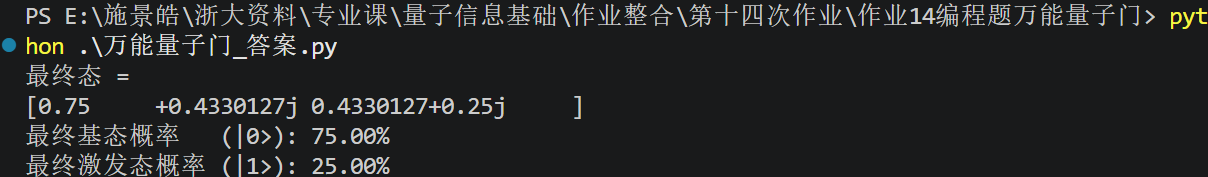
\includegraphics[width=0.95\linewidth]{figures/第一题验证.png}
  \caption{第一问代码验证结果}
  \label{fig:task1_verify}
\end{figure}

\subsection{第二问代码验证：第一个解}

第二问固定
\[
\phi=0,\qquad |\psi_0\rangle=\frac{1}{\sqrt{2}}\left(|0\rangle+i|1\rangle\right).
\]
先取第一个解
\[
\theta=-\frac{\pi}{6}.
\]
在参考代码中，将参数和初始态改为
\begin{lstlisting}
theta = -np.pi / 6
phi = 0.0
state = np.array([1.0 + 0.0j, 1.0j]) / np.sqrt(2)
\end{lstlisting}
运行结果如图 \ref{fig:task2_case1_verify} 所示，最终基态概率为 $25.00\%$，第一激发态概率为 $75.00\%$。这验证了 $\theta=-\pi/6$ 是满足题目要求的解。

\begin{figure}[htbp]
  \centering
  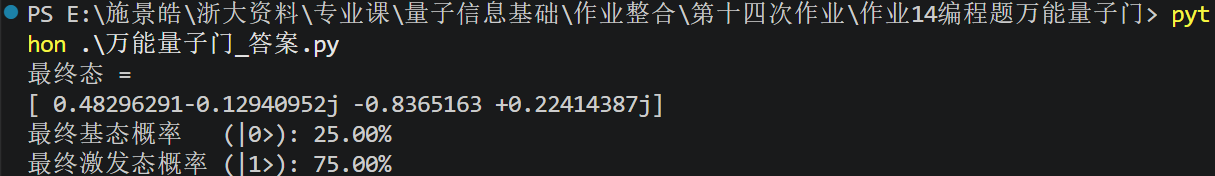
\includegraphics[width=0.95\linewidth]{figures/第二题第一种情况验证.png}
  \caption{第二问第一个解的代码验证结果}
  \label{fig:task2_case1_verify}
\end{figure}

\newpage
\subsection{第二问代码验证：第二个解}

再取第二个解
\[
\theta=-\frac{5\pi}{6}.
\]
在参考代码中，将参数和初始态改为
\begin{lstlisting}
theta = -5 * np.pi / 6
phi = 0.0
state = np.array([1.0 + 0.0j, 1.0j]) / np.sqrt(2)
\end{lstlisting}
运行结果如图 \ref{fig:task2_case2_verify} 所示，最终基态概率为 $25.00\%$，第一激发态概率为 $75.00\%$。这验证了 $\theta=-5\pi/6$ 同样满足题目要求。

\begin{figure}[htbp]
  \centering
  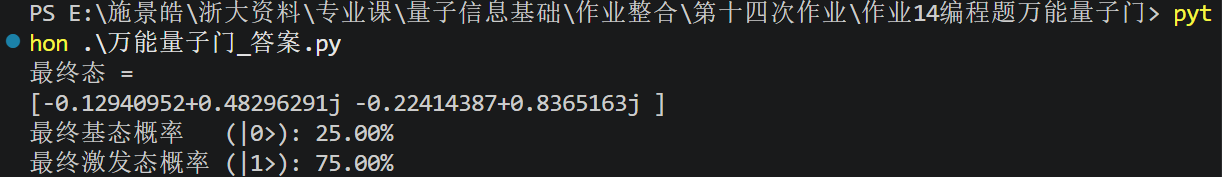
\includegraphics[width=0.95\linewidth]{figures/第二题第二种情况验证.png}
  \caption{第二问第二个解的代码验证结果}
  \label{fig:task2_case2_verify}
\end{figure}

综上，Python 数值验证结果与前两问的理论推导完全一致。第三问题目说明不需要代码验证，因此这里只给出理论推导结论。

\end{document}
